\appendix
\section{Sampling from Watershed}
\label{sec: appendix1}

 During training, the sparse optical flow $\mathbf{P}_{d}$ is sampled from the target optical flow. For effective propagation, those guidance vectors should be placed at some keypoints where the motions are representative. We adopt a watershed-based~\citep{zhan2019self} method to sample such keypoints. Given the optical flow of an image, we first extract motion edges using a Sobel filter. Then we assign each pixel a value to be the distance to its nearest edge, resulting in the topological-distance watershed map. Finally, we apply Non-maximum Suppression (NMS) with kernel size $K_f$ on the watershed map to obtain the keypoints. We can adjust $K_f$ to control the average number of sampled points. A larger $K_f$ results in sparser samples. Points on image borders are removed. With the watershed sampling strategy, all the keypoints are roughly distributed on the moving objects.


\begin{figure}[t]
    \centering
    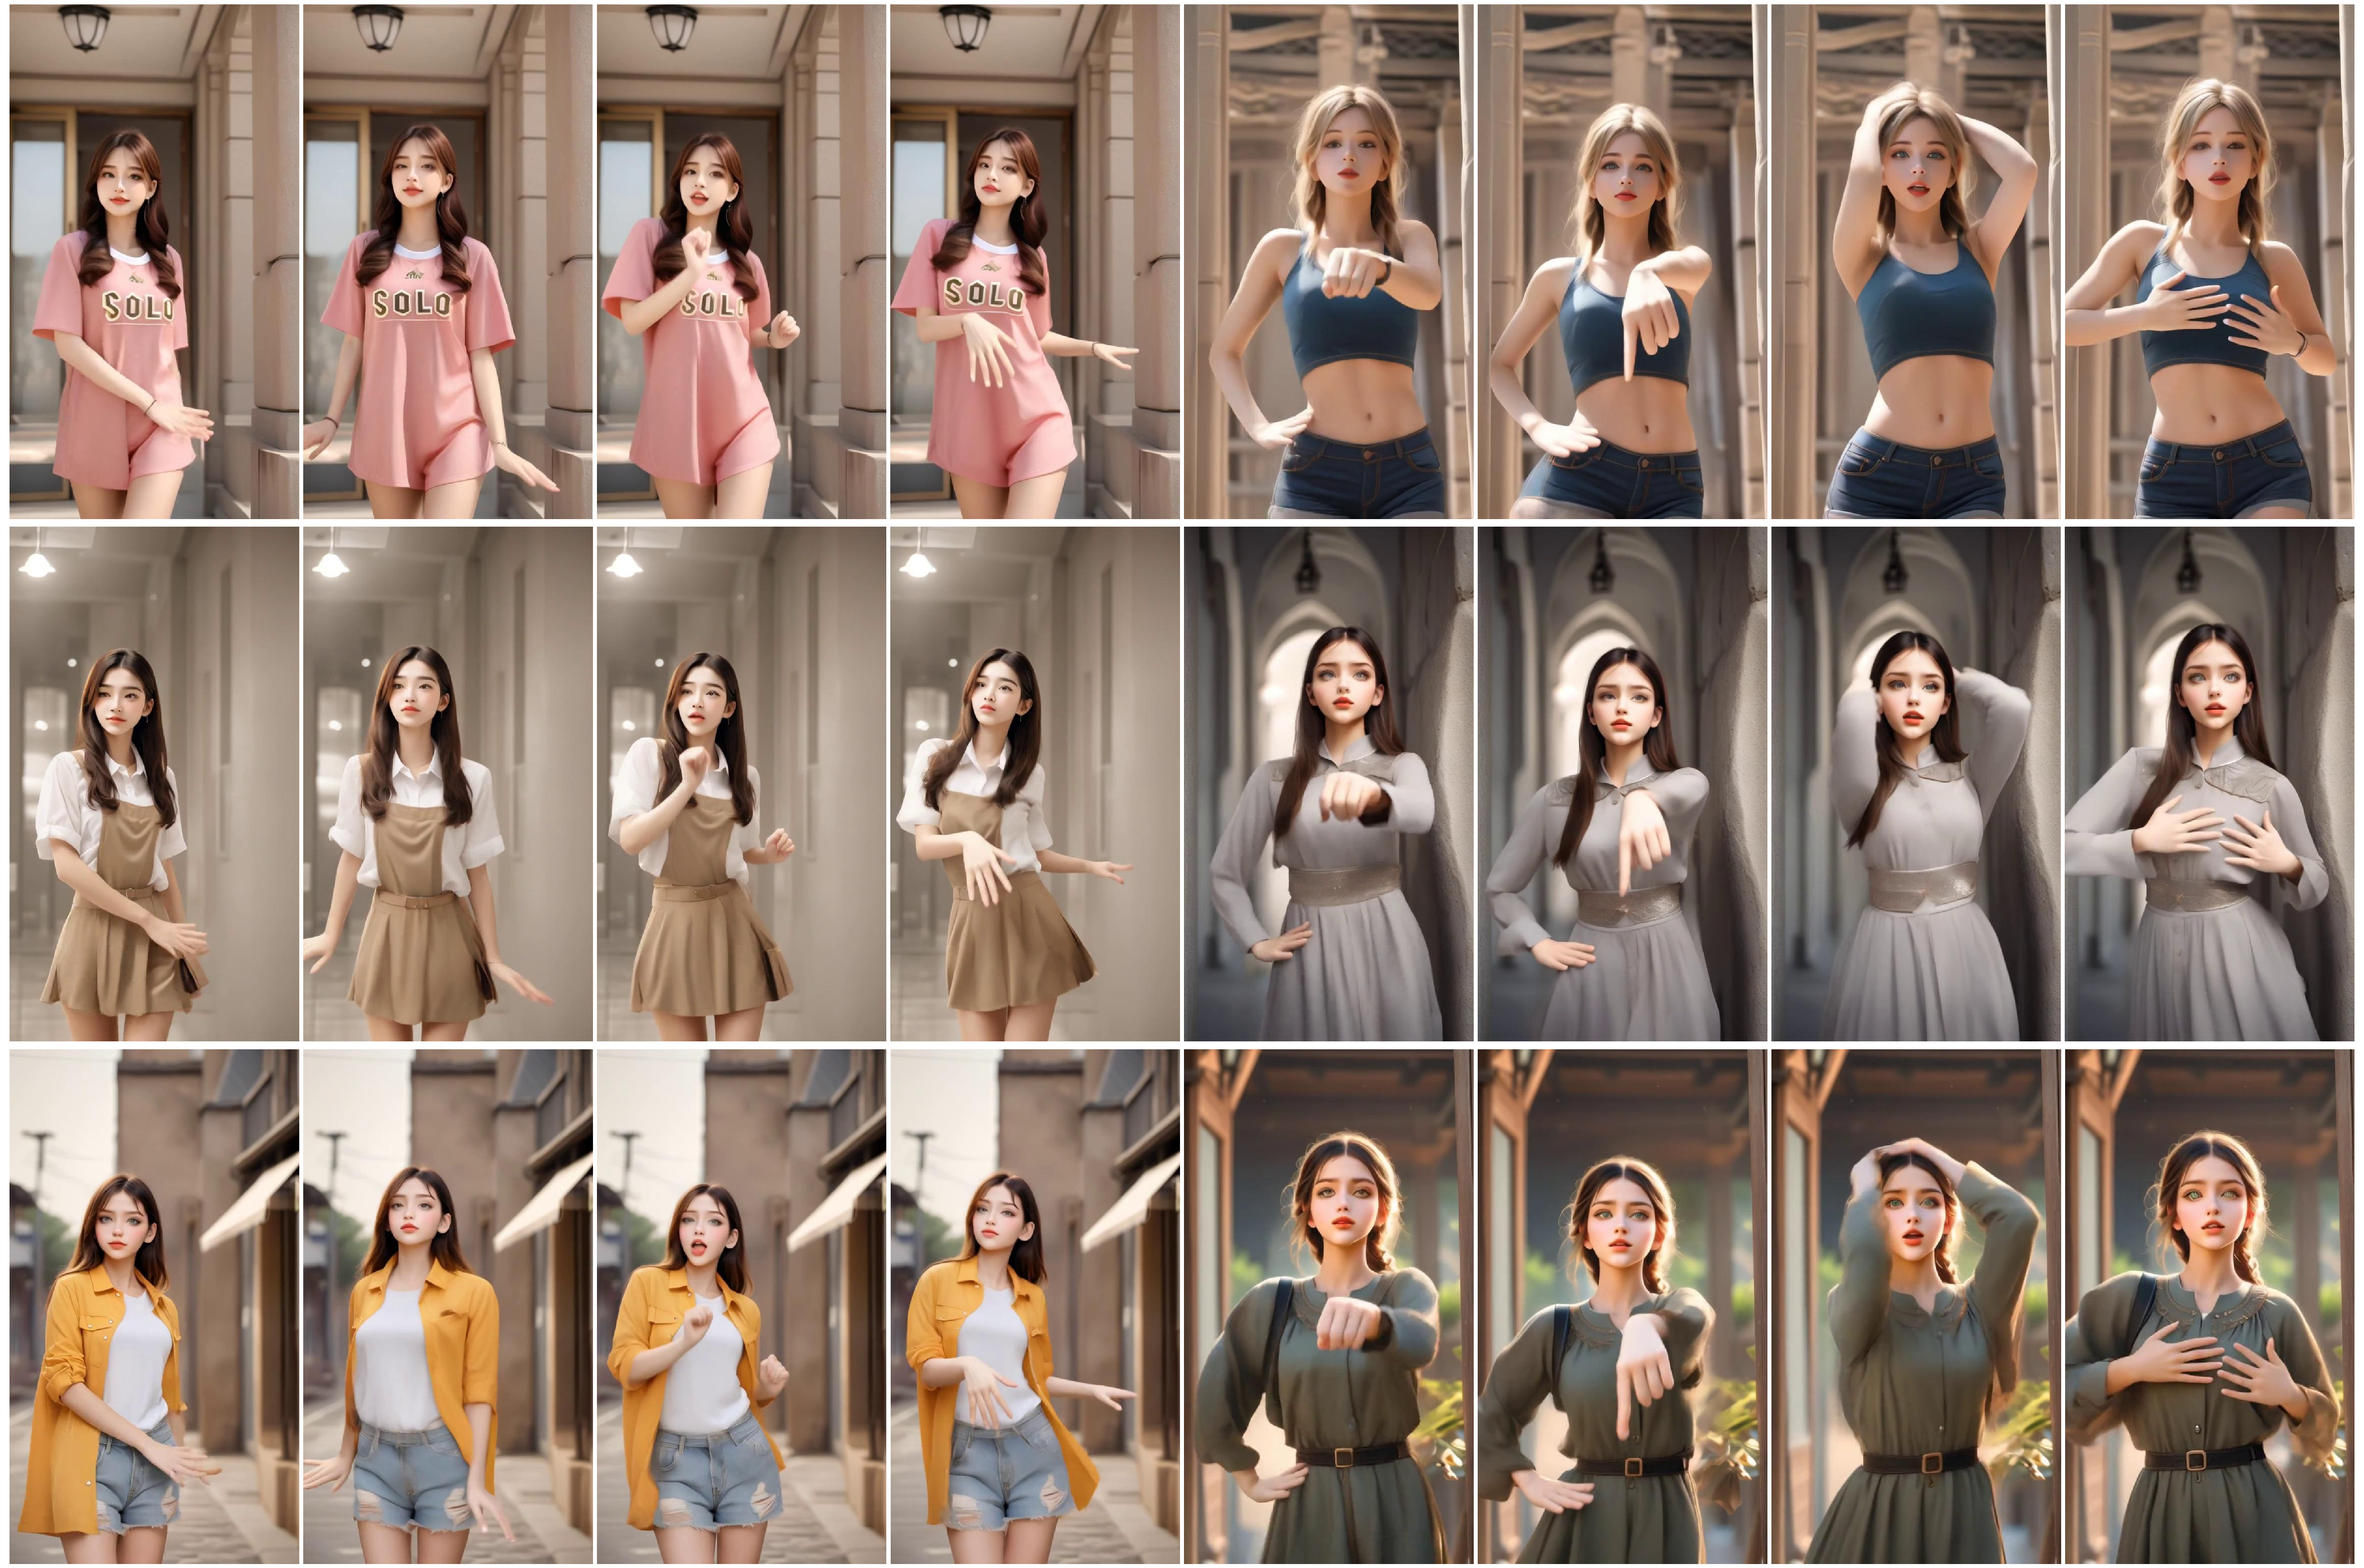
\includegraphics[width=1.0\columnwidth]{./image/appendix_fig1.pdf}
    \vspace{-15pt}
    \caption{More Qualitative Comparisons.}
    \label{fig: appendix_fig1}
\end{figure}

\begin{figure}[t]
    \centering
    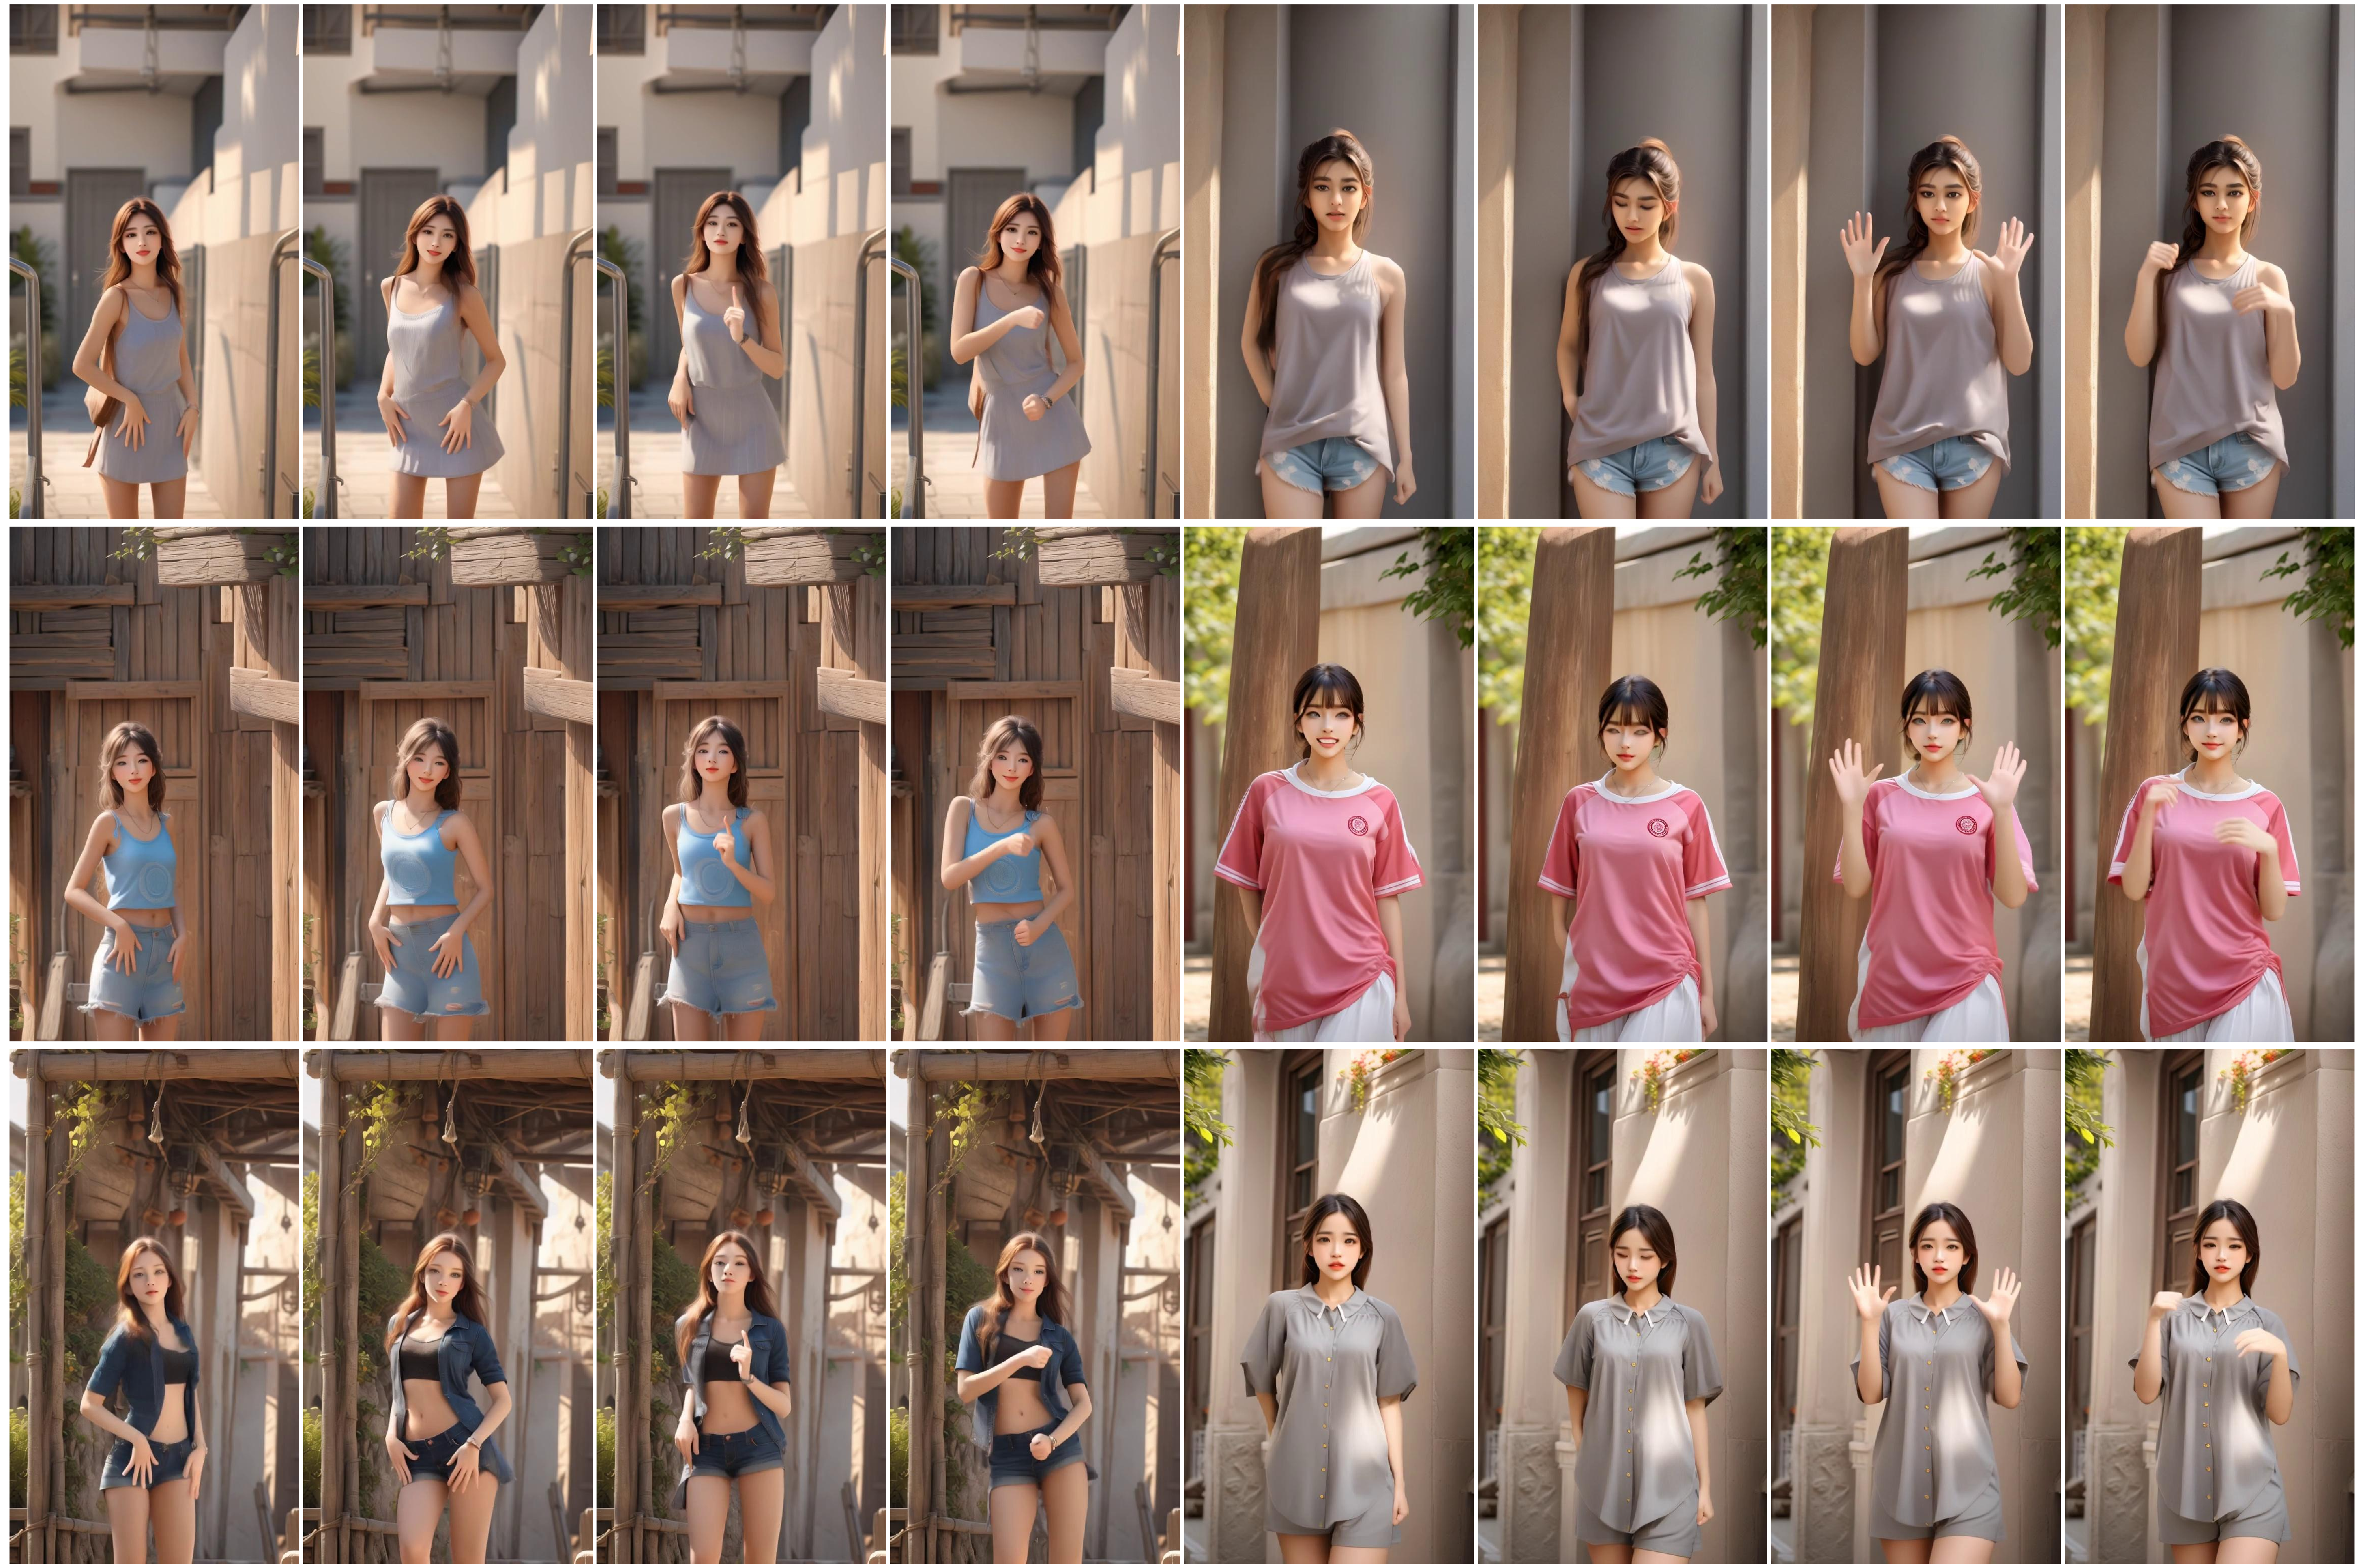
\includegraphics[width=1.0\columnwidth]{./image/appendix_fig2.pdf}
    \vspace{-15pt}
    \caption{More Qualitative Comparisons.}
    \label{fig: appendix_fig2}
\end{figure}
 \section{More Quantitative Results}
 
 Figures~\ref{fig: appendix_fig1} and Figure~\ref{fig: appendix_fig2} illustrate more qualitative results.
\label{sec: more case}

{
\section{More Ablation Analyses}
As shown in Figure~\ref{fig: appendix abs}, the region-level guidance provided by our motion field guidance facilitates the enhancement of consistency across body regions. The proposed keypoints correspondence improves generation quality by aligning DIFT features of the skeleton pose, e.g., facial consistency.
 }

 \begin{figure}[t]
    \centering
    \includegraphics[width=1.0\columnwidth]{./image/abs.png}
    \caption{Qualitative results about motion field guidance and keypoints correspondence.}
    \vspace{-10pt}
    \label{fig: appendix abs}
    
\end{figure}

{
\section{More details of motion field guidance}
There is a gap between the inference and the training optical flow. 
(1) During inference, we do not propose extracting the forward optical flow directly from the driving video, as it ignores the gap between the reference character and the driving video. As shown in Figure~\ref{fig: appendix_flow1}(a)and Figure~\ref{fig: appendix_flow2}(a), directly using the forward optical flow as motion guidance is clearly inconsistent with the reference image.
(2) When there is a large difference between the reference image and the driving video, it is impossible to get the corresponding motion field by the existing optical flow estimation model, as shown in Figure~\ref{fig: appendix_flow2}(b). Therefore, we have to compute Pd differently during inference.
}
{
Although the dense motion field we proposed in Section 4.1 can adapt to different body variations during inference. However, there are two limitations of this dense motion field: (1) there is a gap with the motion field extracted from real videos, and (2) the low computational efficiency is not suitable for use during training. Considering that pairs of training data have no body changes, to utilize accurate control signals during training and to improve computational efficiency, we approximate the optical flow during inference by sampling sparse optical flow before prediction as shown in Figure~\ref{fig: appendix_flow1}(c). 
}

% ############################################
\begin{table*}[t]
\footnotesize
\begin{minipage}[t]{0.33\textwidth}
\centering
\setlength{\tabcolsep}{2pt}
\caption{The impact of hybrid ControlNet.}
% \vspace{-10pt}
\begin{tabular}{lcc}
\toprule
{Methods} & FID-FVD$\downarrow$   & FVD$\downarrow$\\ 
\midrule
Exp1 & 10.43 & 514.83 \\
Exp2 & 10.94 & 551.32 \\
Full Model & 10.24 & 466.93 \\
 \bottomrule
\end{tabular}
\label{tab:appendix_controlnet}
\end{minipage}
\hfill
\begin{minipage}[t]{0.65\textwidth}
\caption{The impact of CMP.}
% \vspace{-10pt}
\centering
\setlength{\tabcolsep}{2pt}
\begin{tabular}{lcc}
\toprule[1pt]
Methods  & subject consistency$\uparrow$ & background consistency$\uparrow$ \\
\midrule
Full Model w/o CMP & 93.94                  &   97.83\\            
Full Model         &94.35                  &  98.75   \\
\bottomrule
\end{tabular}
% \vspace{-1pt}
\label{tab:appendix_cmp}
\end{minipage}
% \vspace{-5pt}
\end{table*}

\begin{table}[t]
% \vspace{-10pt}
\caption{Performance comparisons for image-level metrics.}
\centering
% \setlength{\tabcolsep}{3pt}
\begin{tabular}{lcccc}
\toprule
Methods  & SSIM $\downarrow$ & PSNR$\downarrow$ & LPIPS$\uparrow$  & L1$\uparrow$ \\
\midrule
MusePose &0.788& 19.14&  0.263&  2.46E-05\\     
MusePose+Ours  &0.811  &19.36  &0.238  &2.26E-05\\
\midrule
MimicMotion &0.749  &18.32  &0.272& 2.71E-05\\
MimicMotion+Ours & 0.781&19.58 &0.242&2.42E-05 \\
\bottomrule
\label{tab:appendix_exp}
\end{tabular}
\end{table}

\begin{table}[t]
% \vspace{-10pt}
\caption{Performance comparisons for image-level metrics.}
\centering
% \setlength{\tabcolsep}{3pt}
\begin{tabular}{lcc}
\toprule
Methods  & trainable parameters(MB) & infer time (sec/frame) \\
\midrule
MusePose	&2072.64	&3.37 \\
MimicMotion	&1454.19	&1.61 \\
MimicMotion+Ours	&653.4	&2.36\\
\bottomrule
\label{tab:appendix_eff}
\end{tabular}
\end{table}

{
\section{More Ablation Study}
\subsection{The impact of hybrid ControlNet architecture}
We show the impact of hybrid ControlNet architecture in Table~\ref{tab:appendix_controlnet}. Specifically, we design two variant architectures, (1) Exp1: inserting the motion field into the denoising network instead of the hybrid controller as shown in Figure~\ref{fig: appendix_abs_pipeline}(a), and (2) Exp2: removing the hybrid ControlNet and inserting the motion field guidance and keypoint correspondence into the denoising network as shown in Figure~\ref{fig: appendix_abs_pipeline}(b). Exp1 shows that the motion field needs to be jointly optimized with U-Net to provide the correct representation. Exp2 shows that complex motion information and appearance features cannot be modeled with only two shallow encoders.
}
{
\subsection{The impact of CMP.}
We provide the ablation analysis of CMP in Table~\ref{tab:appendix_cmp}, which shows that CMP can improve the consistency of the generated video.
}

\begin{figure}[h!]
    \centering
    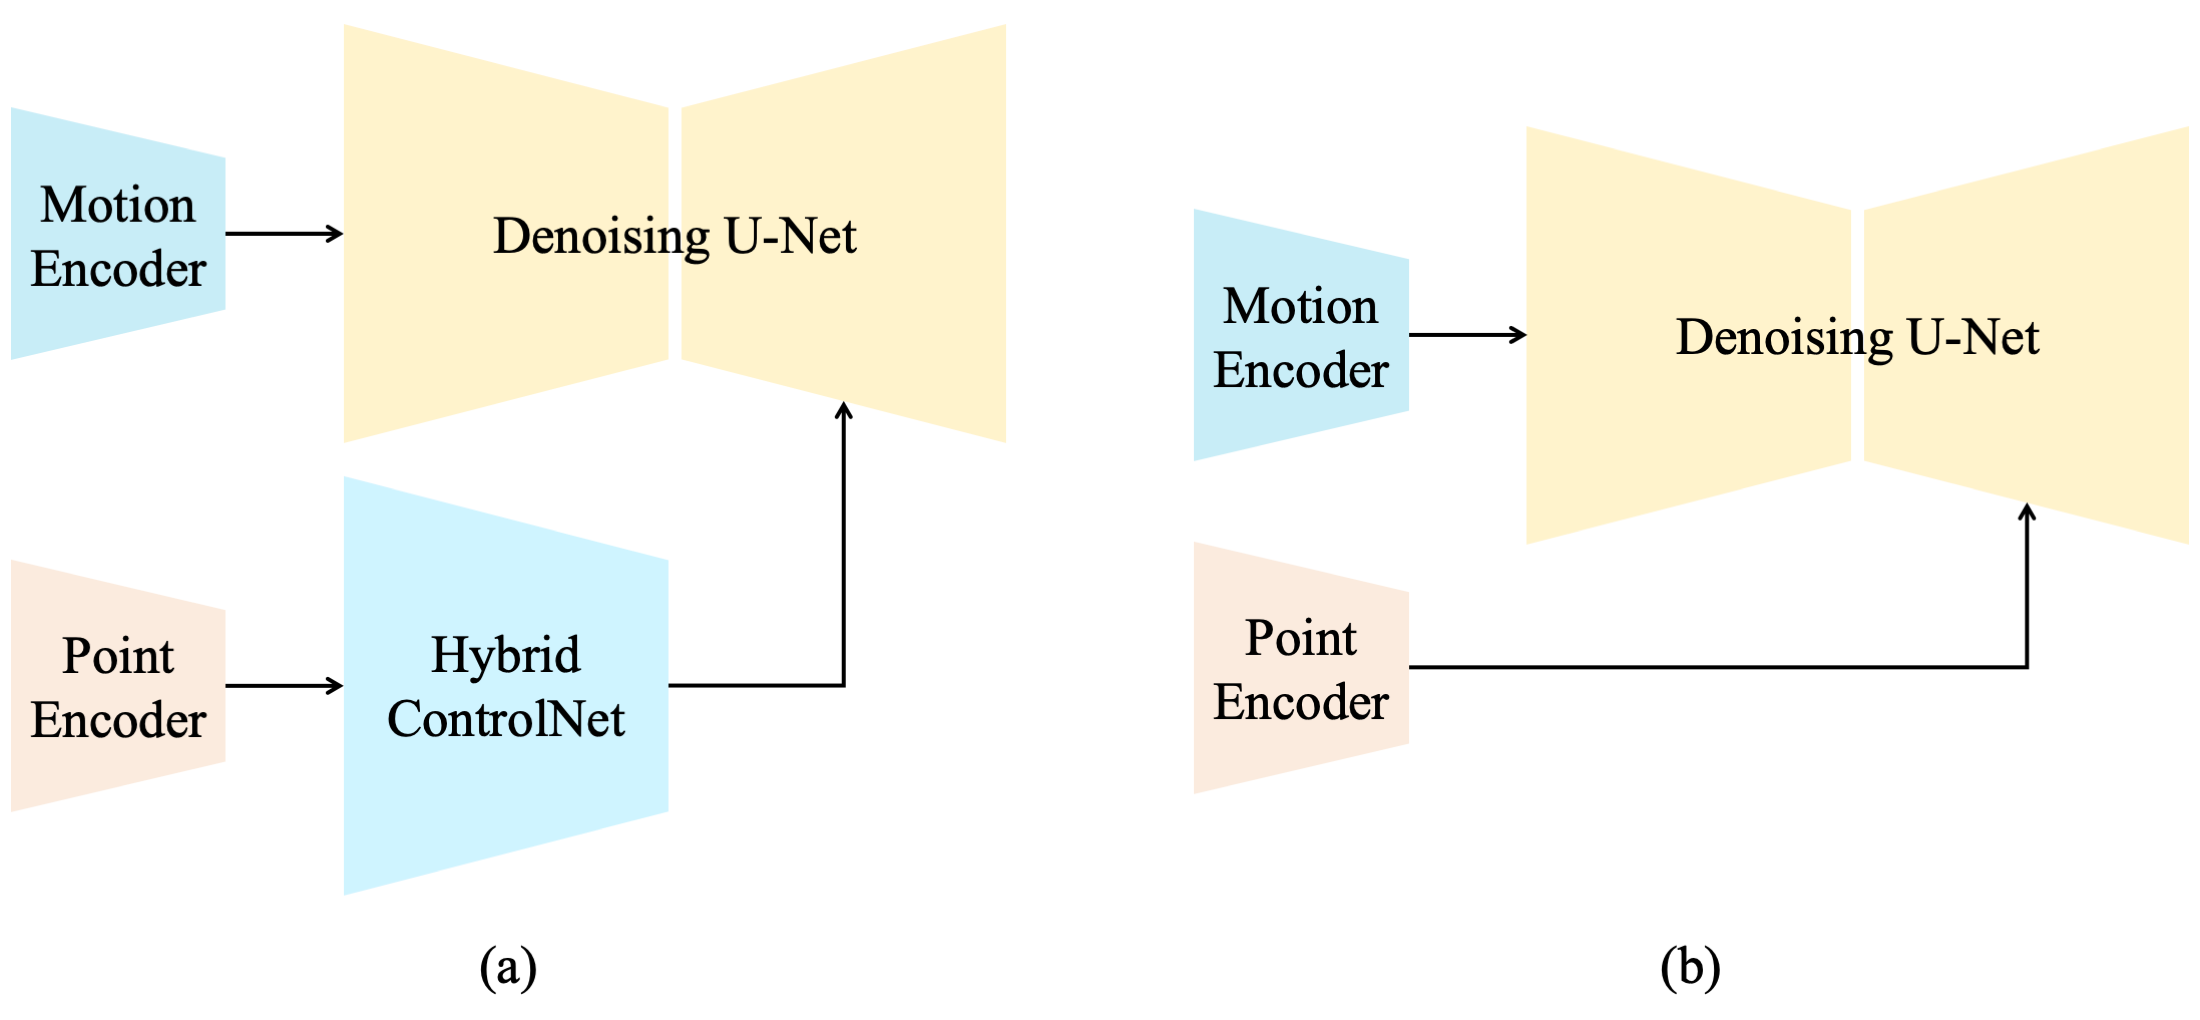
\includegraphics[width=.9\columnwidth]{./image/abs_pipeline.png}
    \vspace{-15pt}
    \caption{Different hybrid ControlNet architectures.}
    \label{fig: appendix_abs_pipeline}
\end{figure}

{
\section{More Performance Comparisons.}
To further evaluate the generated results, we provide performance comparisons for image-level metrics in Table~\ref{tab:appendix_exp}. Compared to the baseline model, our method achieves significant improvements in all metrics.
}
{
\section{Trainable Parameters and Inference Time}
We compare the trainable parameters and inference time of the different models in Table~\ref{tab:appendix_eff}. For a fair comparison, the size of the generated video is set to 576x1024. Our method requires fewer trainable parameters based on the baseline model.
During inference, our method estimates the motion field for the reference image, which increases inference time a little.
}

{
\section{Analysis of Background Noise.}
Since our motion fields are not extracted directly from the driving video, some noise due to estimation errors may be introduced. As shown in Figure~\ref{fig: appendix_flow_noise}, the motion field of the reference image without the background is more accurate than the complex background.
}

\begin{figure}[t]
    \centering
    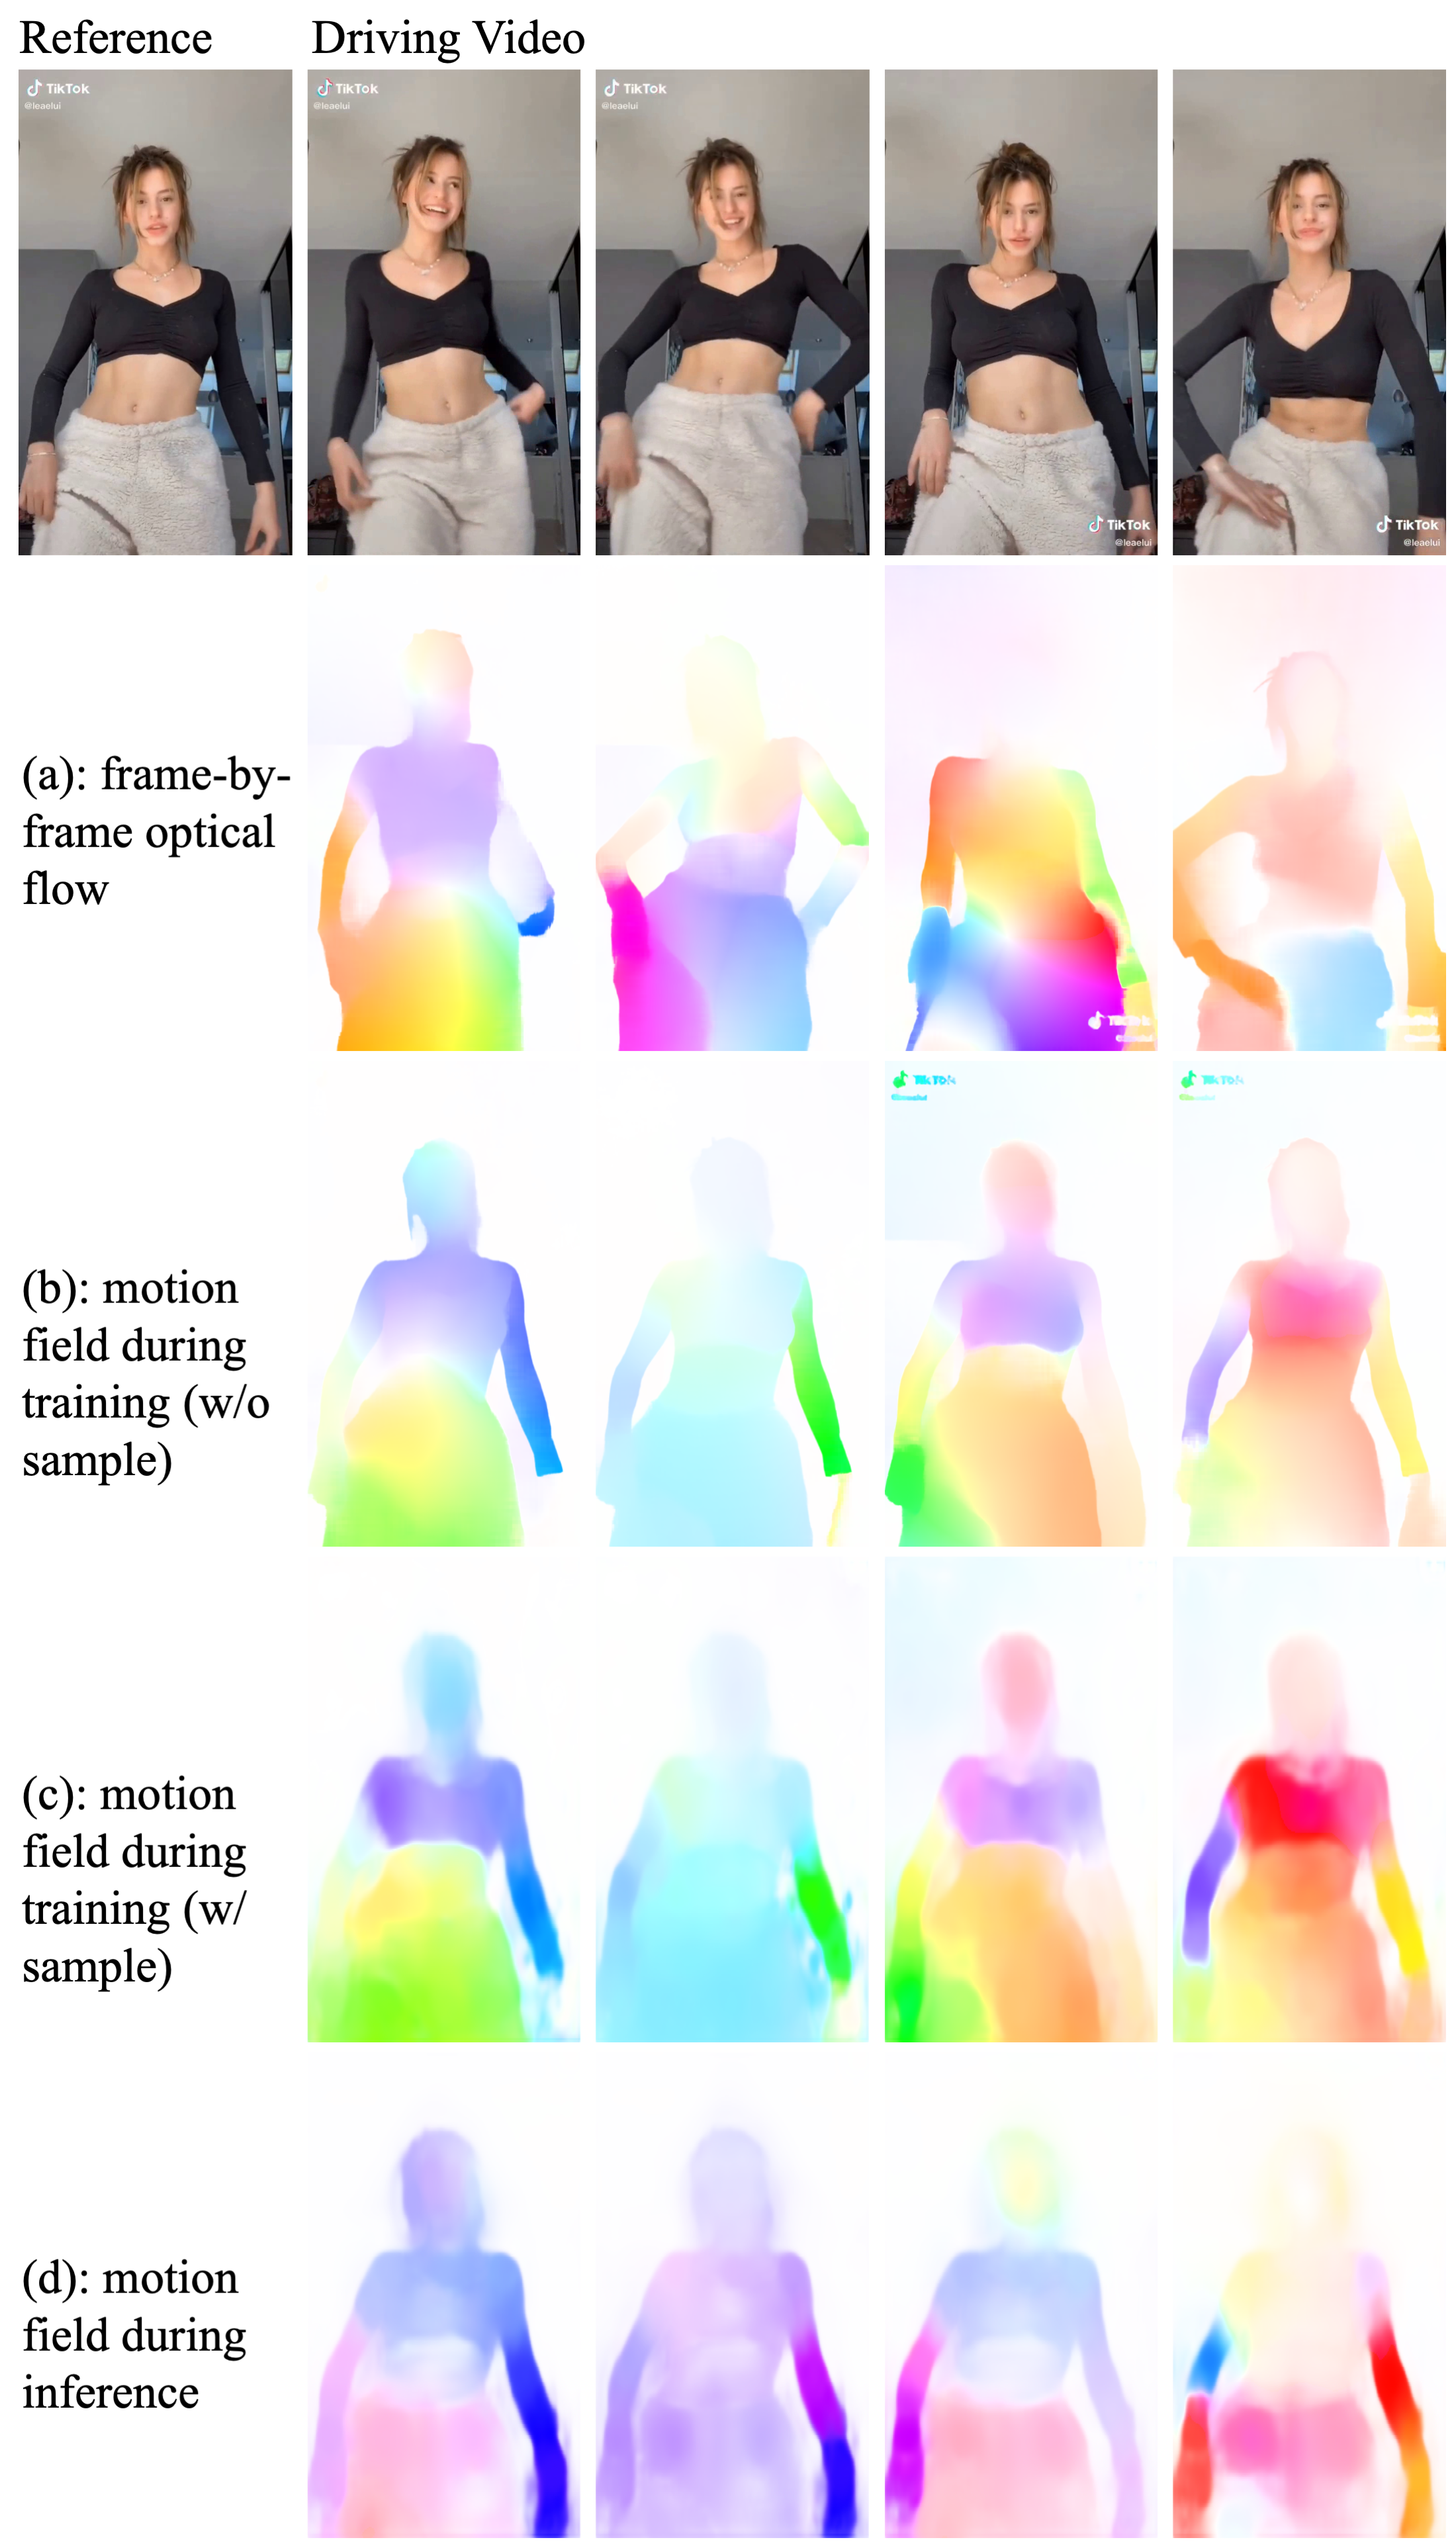
\includegraphics[width=.9\columnwidth]{./image/flow1.png}
    \vspace{-10pt}
    \caption{Body matched motion field visualization.}
    \label{fig: appendix_flow1}
\end{figure}

\begin{figure}[t]
    \centering
    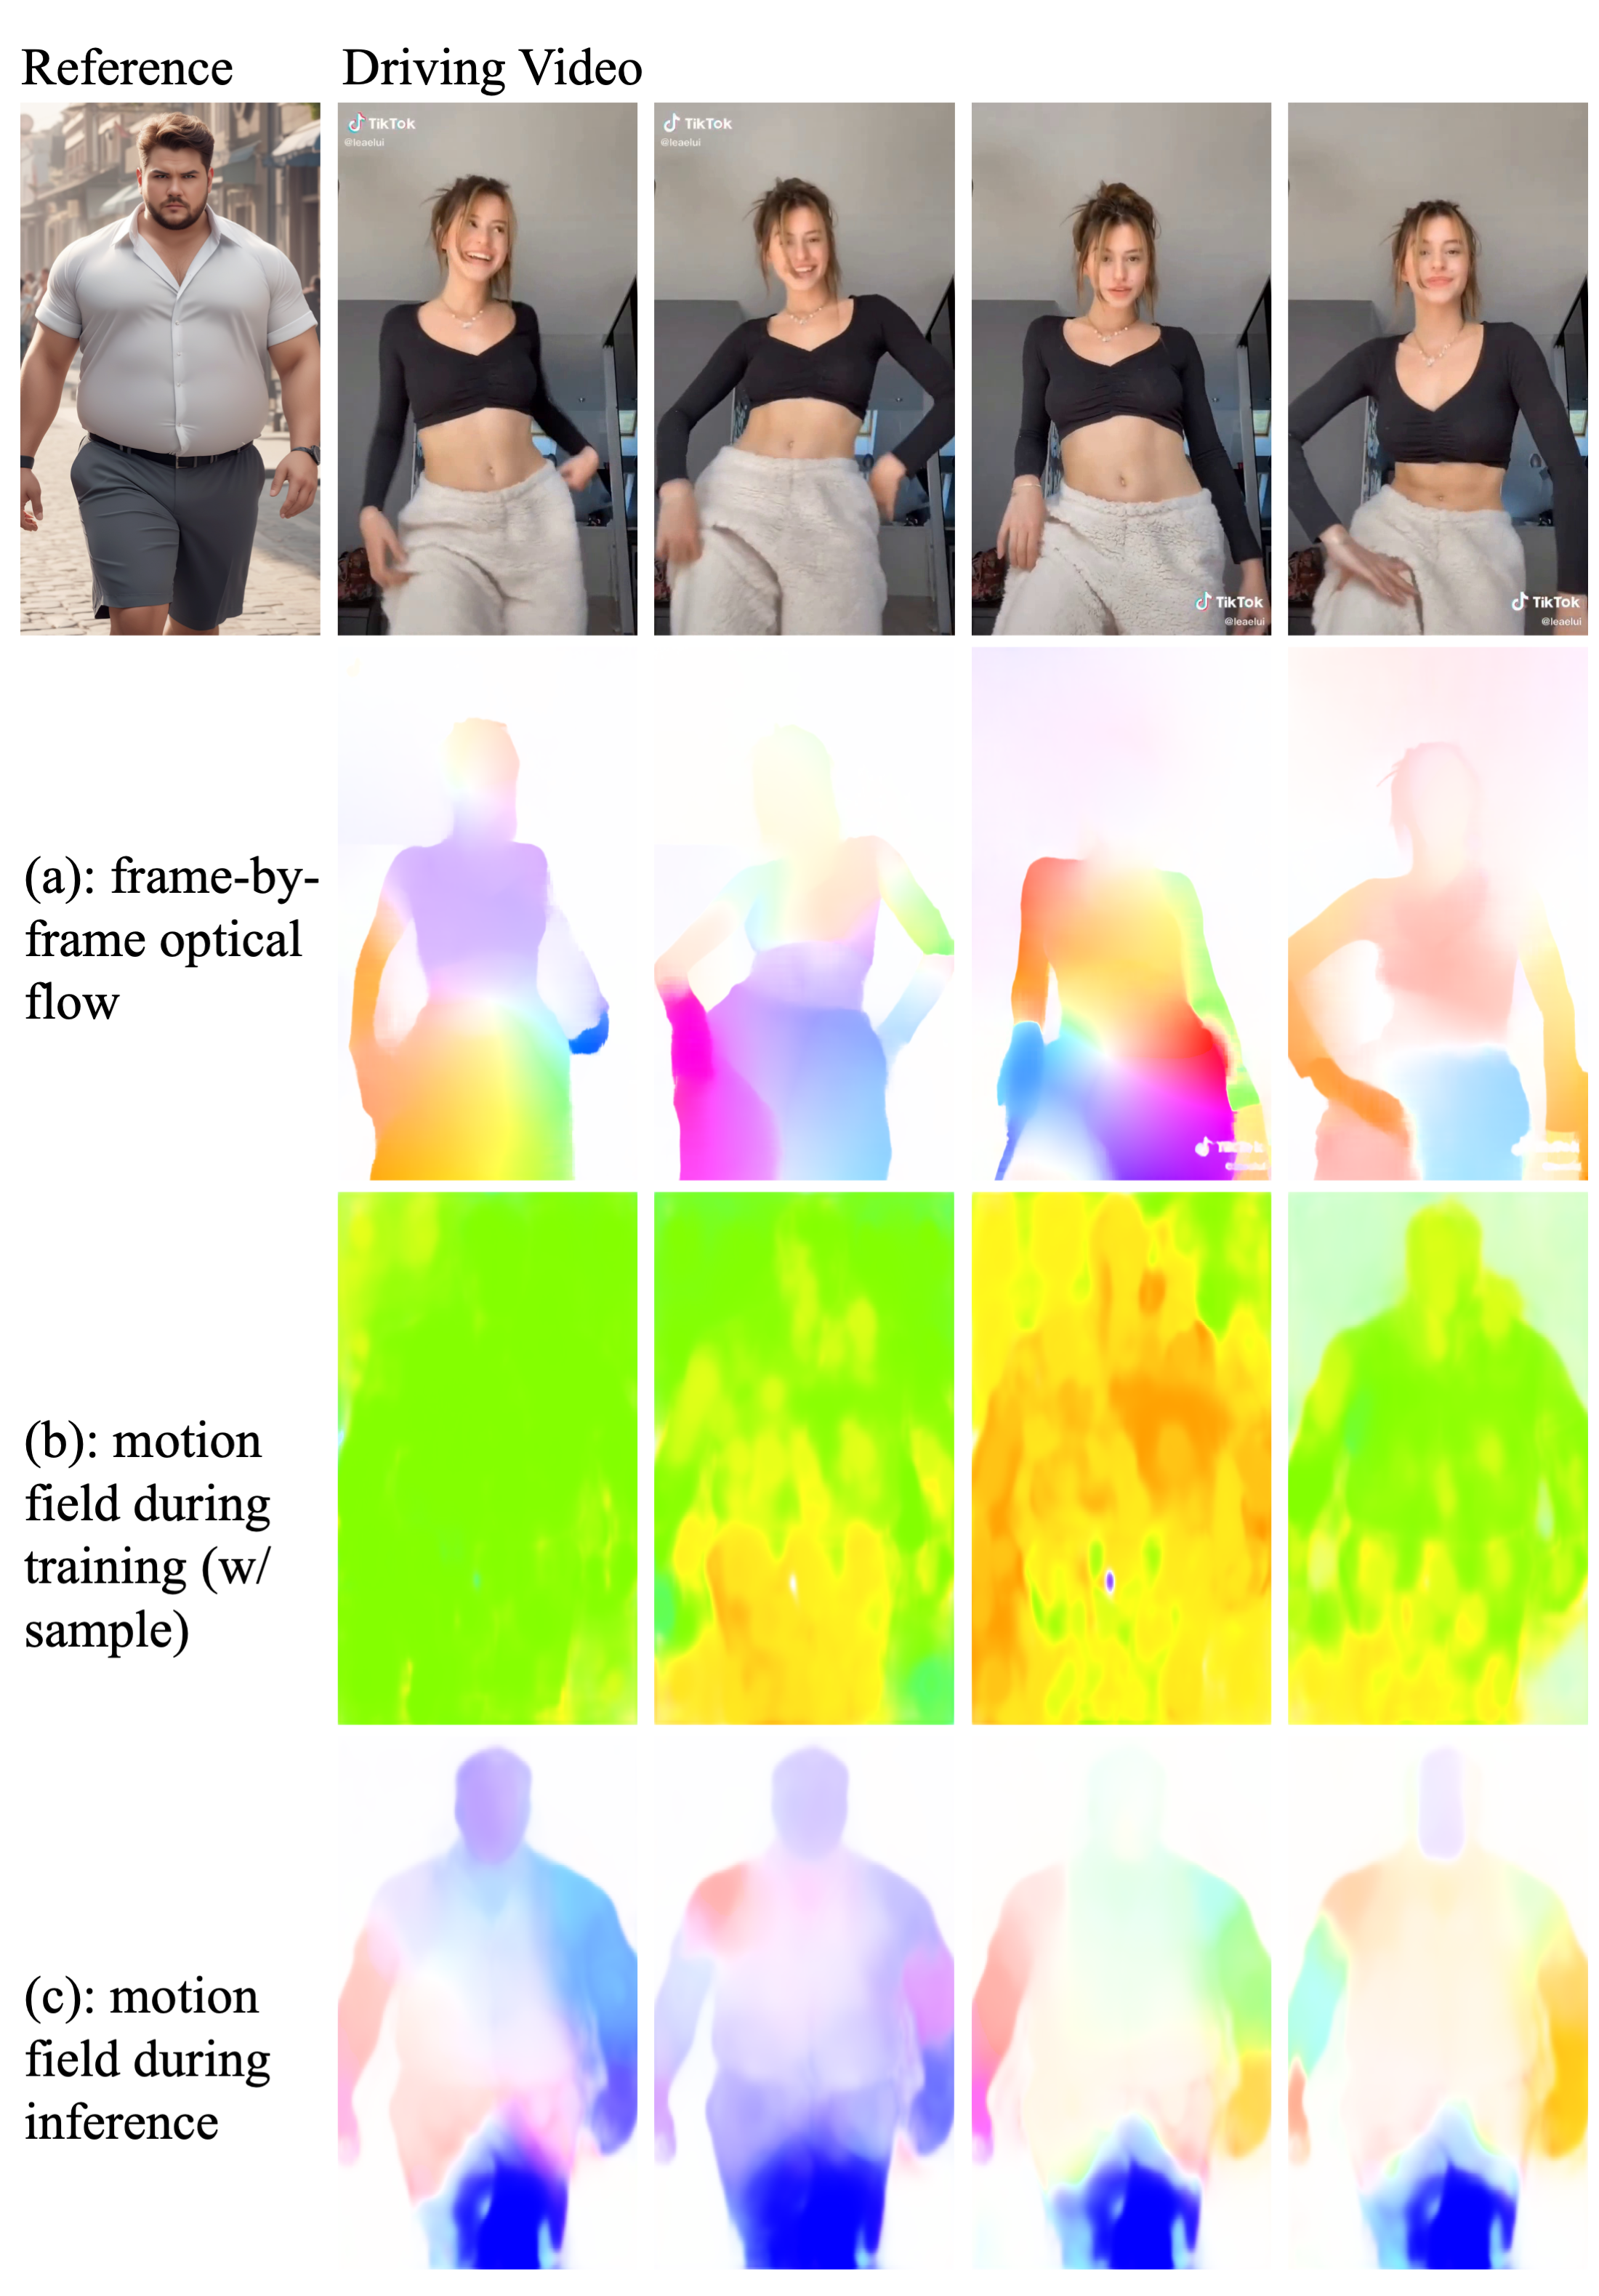
\includegraphics[width=.9\columnwidth]{./image/flow2.png}
    \vspace{-10pt}
    \caption{Body mismatched motion field visualization.}
    \label{fig: appendix_flow2}
\end{figure}

\begin{figure}[t]
    \centering
    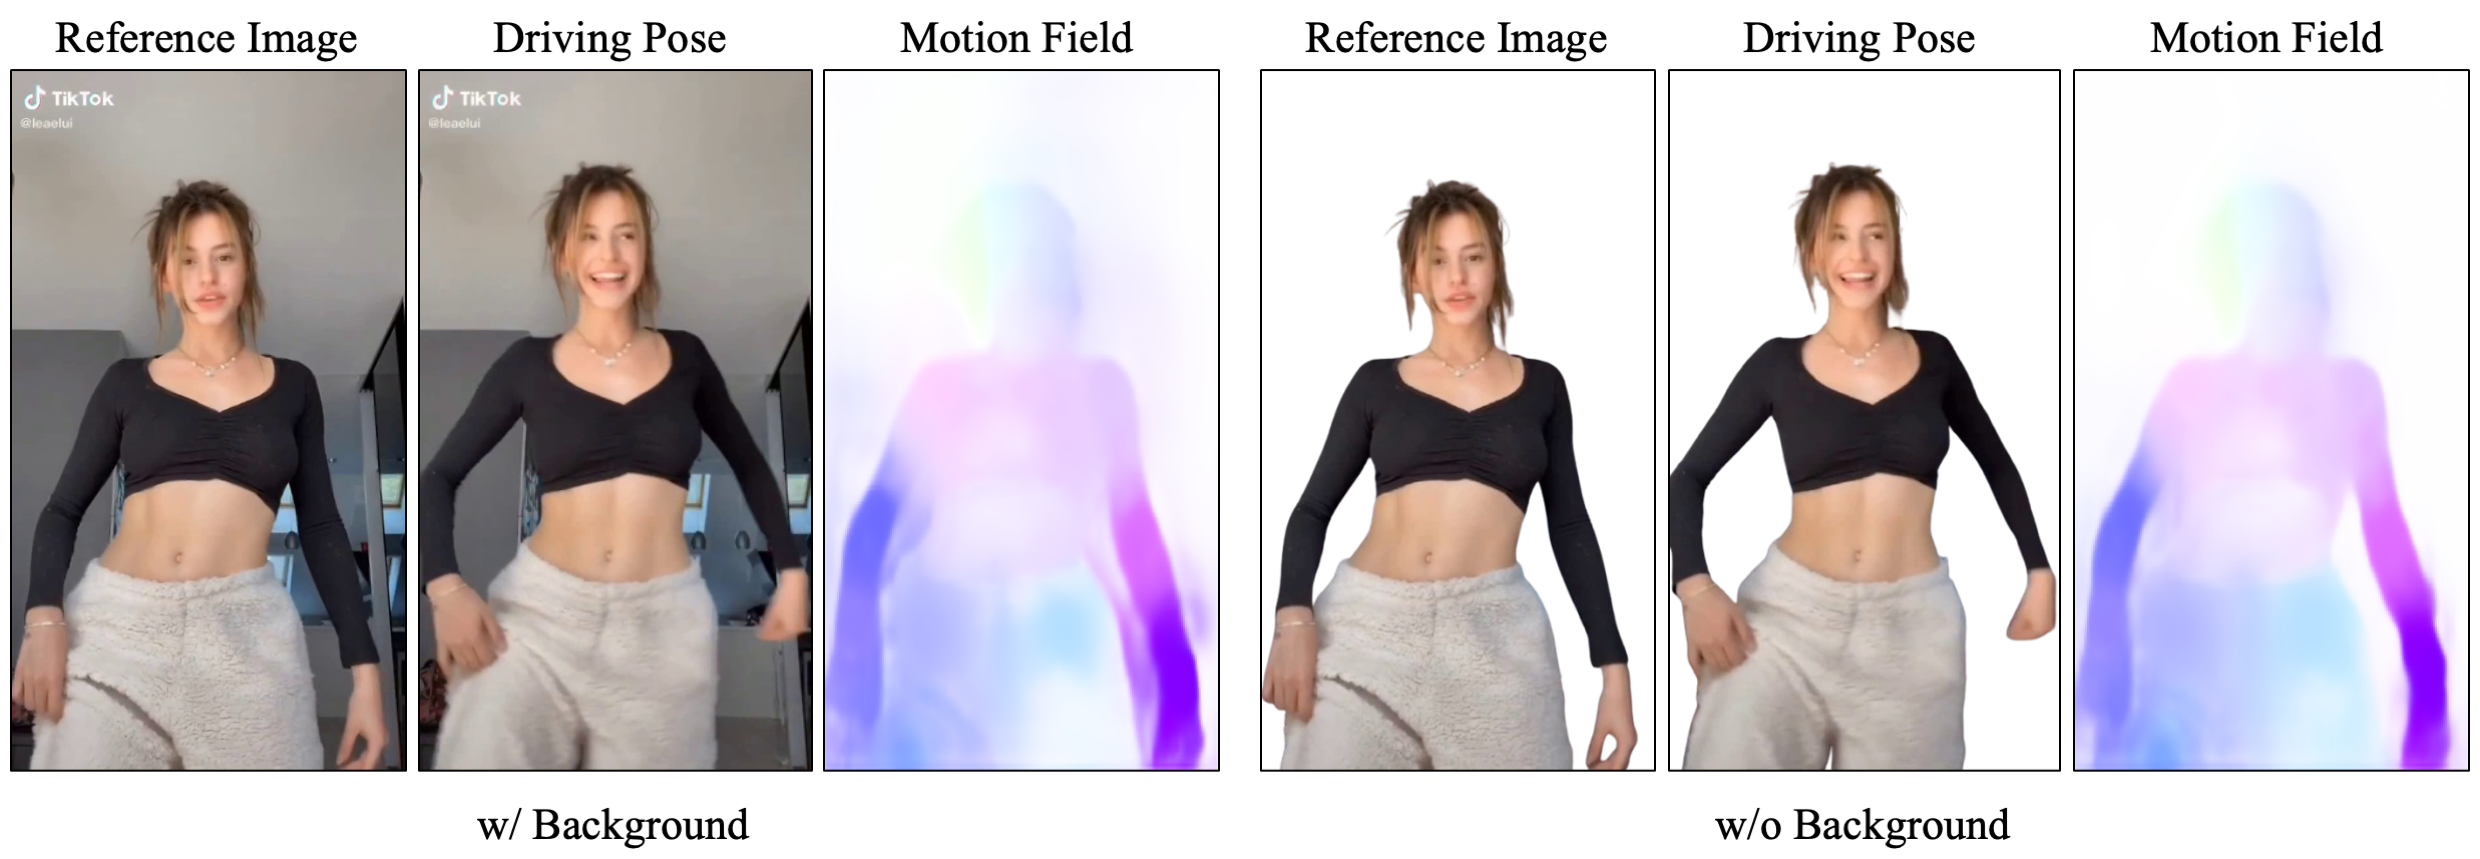
\includegraphics[width=.9\columnwidth]{./image/flow_noise.png}
    \vspace{-10pt}
    \caption{Analysis of background noise.}
    \label{fig: appendix_flow_noise}
\end{figure}